\subsection{Modelado CAD para prototipo}
En esta sección se muestran los diseños implementados y utilizados en el prototipo, a diferencia de los diseños propuestos antes, estos cuentan con canales para el pasaje de los cables y con detalles que surgieron de las distintas impresiones y pruebas previas que guiaron hacia el resultado y diseño final de cada soporte para la implementación en el prototipo.
\subsubsection{Suporte superior}
El soporte superior (fig. \ref{fig:Superior_orginal}) es el que recibe la mayor carga en la estructura, ya que debe soportar el peso de la estructura vertical (soportes, brazo robótico, varillas). Para ello se debe realizar un analisis de carga y deformación previos para verificar si la forma del soporte es la adecuada para tolerar los esfuerzos.
\begin{figure}[H]
    \centering
    \begin{subfigure}[b]{0.35\textwidth}
        \centering
        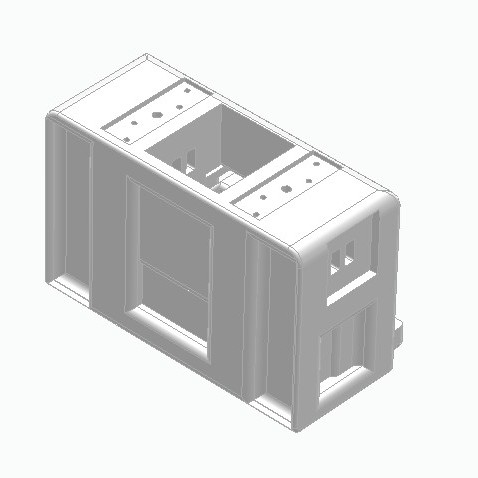
\includegraphics[width=0.75\textwidth]{img/Superior_frente.jpg}
        \caption{Frente del soporte superior.}
        \label{fig:izaje_desacoplado}
    \end{subfigure}
    \hspace{0.02\textwidth}
    \begin{subfigure}[b]{0.35\textwidth}
        \centering
        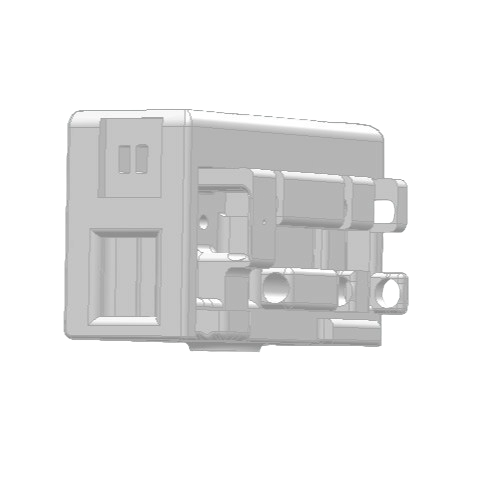
\includegraphics[width=0.75\textwidth]{img/superior_atras.jpg}
        \caption{Posterior del soporte superior.}
        \label{fig:izaje_acoplado}
    \end{subfigure}
     \caption{Soporte superior.}
    \label{fig:Superior_orginal}
\end{figure}
Para realizar el análisis de esfuerzos y deformación se simplificó la pieza ya que el solver del software utilizado no podía procesar y analizar geometrías tan complejas como la planteada. Además se tomaron las propiedades del filamento plástico PETG de impresión 3D para hacer un correcto analisis.\\
En la siguiente figura se pueden observar las fuerzas aplicadas, las mismas contemplan una carga máxima de 3.5kg. Las fuerzas son aplicadas en las secciones indicadas en la imagen y dividas en dos para la parte superior y en tres para la parte inferior.\\
\begin{figure}[H]
    \centering
        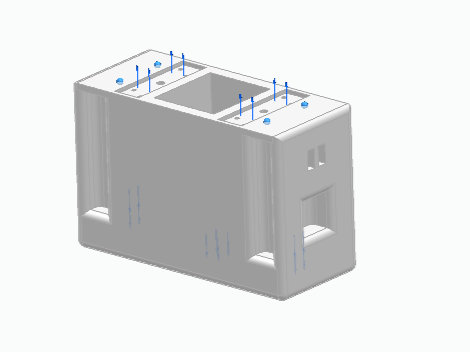
\includegraphics[width=0.5\textwidth]{img/Fuerzas_superiores.png} \par
        \caption{\textit{Fuerzas aplicadas para el análisis}}
        \label{fig:fuerzas_sup}
\end{figure}
%    
%\end{figure} 
Como se puede observar en las imágenes, la tensión está muy por debajo de la tensión de rotura y las deformaciones son prácticamente insignificantes, por lo que se puede concluir que el diseño es aplicable.\\
\begin{figure}[H]
    \centering
    \begin{subfigure}{0.35\textwidth}
        \centering
        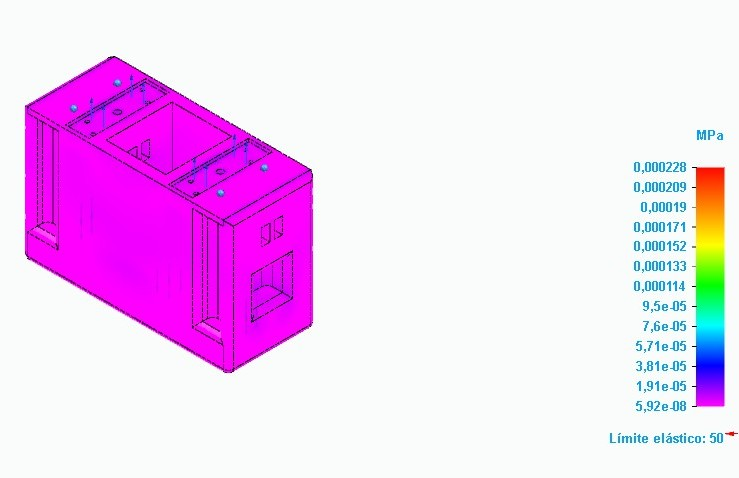
\includegraphics[width=0.8\textwidth]{img/completo_sin_mallar.jpg} \par
        \caption{\textit{Análisis de tensión de Von Misses.}}
        \label{fig:sup_analisis_tension}
    \end{subfigure}
    \hspace{0.5cm}
    \begin{subfigure}{0.35\textwidth}
        \centering
        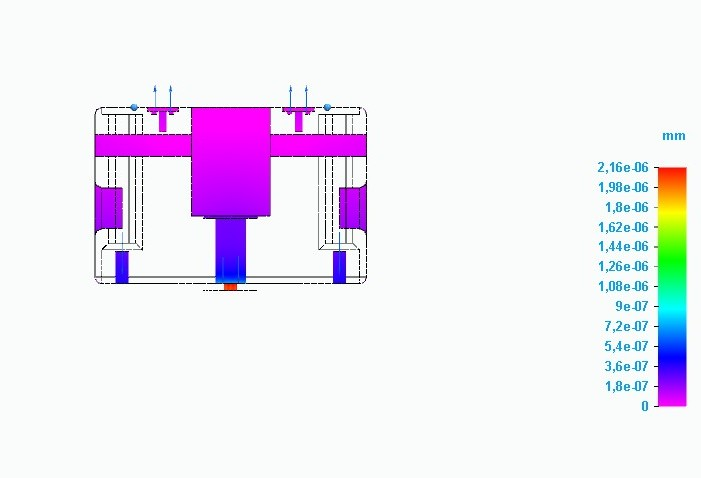
\includegraphics[width=0.8\textwidth]{img/Corte_transv_sin_mallado_def.jpg} \par
        \caption{\textit{Análisis de deformación.}}
        \label{fig:sup_analisis_def}
    \end{subfigure}
    \caption{Soporte superior. Resultados de analisis de esfuerzos y deformaciones.}
\end{figure}

\subsubsection{Suporte medio}
Este soporte se desplaza por el movimiento de la varilla, además es en donde se encuentra el brazo robótico y la cámara. Cuenta con canales internos para el montaje de los cables. \\
\begin{figure}[H]
    \centering
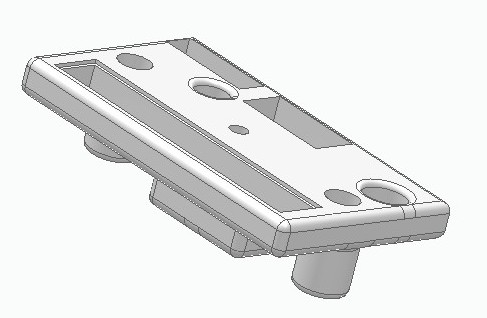
\includegraphics[width=0.45\textwidth]{img/medio.jpg} \par
    \caption{\textit{Soporte medio.}}
    \label{fig:soporte_medio}
\end{figure}

\subsubsection{Suporte inferior}
Este soporte cierra la estructura vertical, en el van los extremos de las varillas trefiladas y la varilla roscada y el final de carrera correspondiente. También cuenta con canales internos para el montaje de los cables. \\
\begin{figure}[H]
    \centering
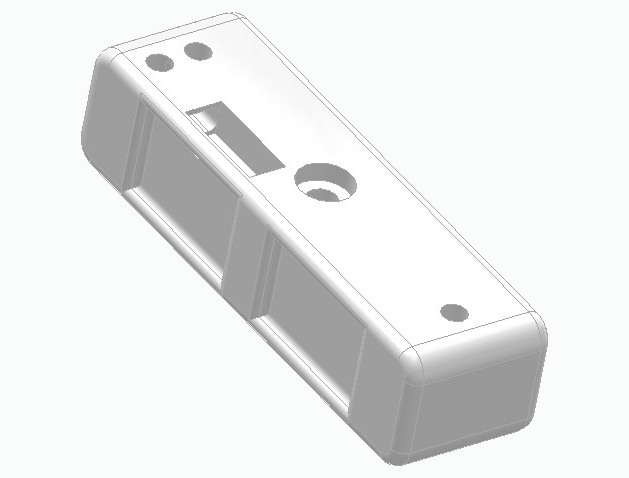
\includegraphics[width=0.45\textwidth]{img/inferior_completo.jpg} \par
    \caption{\textit{Soporte inferior.}}
    \label{fig:soporte_inferior}
\end{figure}

\subsubsection{Robot serie}
Para el diseño del brazo robótico se tienen 2 partes principales, el cuerpo del brazo y el efector final o gripper. \\
El diseño del gripper tiene en cuenta un sistema de transmisión piñon-cremallera para el agarre, igual que el de la  fig. \ref{fig:gripper_Real_transmision}. La diferencia entre ambos robots serie no radica en el diseño si no en el material. Este brazo se plantea para ser impreso en PETG/PLA.\\

\begin{figure}[H]
    \centering
    \begin{subfigure}{0.35\textwidth}
        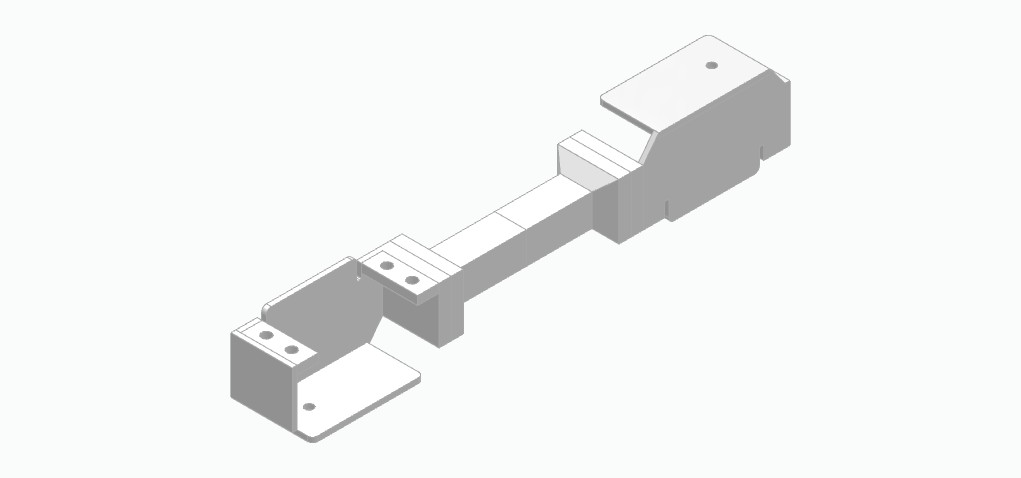
\includegraphics[width=\textwidth]{img/brazo_medio.jpg} \par
    \caption{\textit{Cuerpo del brazo.}}
    \label{fig:brazo}
    \end{subfigure}
    \hspace{0.5cm}
    \begin{subfigure}{0.35\textwidth}
        \centering
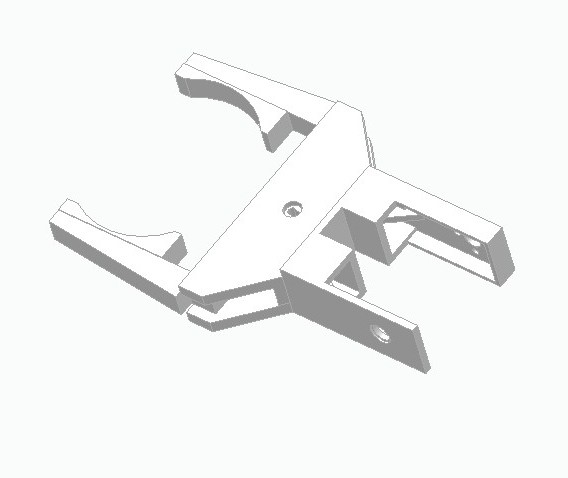
\includegraphics[width=\textwidth]{img/pinza.jpg} \par
    \caption{\textit{Gripper.}}
    \label{fig:gripper}
    \end{subfigure}
    \caption{Piezas principales del robot serie.}
\end{figure}